%!TEX root = ../main.tex

\chapter{Theory\label{chap:theory}}
\section{Radioactive decay}
Radioactive decay is a process where an unstable atomic nucleus transforms into a lower-energy state.
During this process, it loses energy by radiation.
There are three main types of such radiation - alpha, beta and gamma.
Whereas alpha particles can be stopped by a sheet of paper and beta particles by aluminium shielding, gamma particles can be blocked only using a thick block of lead or a massive concrete wall.
Moreover, highly energetic gamma rays have a negative effect on the human body, causing damage on a cellular level.
Being exposed to such radiation poses a risk of severe health problems or death.

\section{Some properties of gamma radiation}
The important property of ionizing radiation is that the intensity of the radiation decreases with the inverse square law.
In other words, the intensity at a given point is proportional to $\frac{1}{d^{2}}$, where $d$ is the distance from the source.
The quantity of emitted particles ("strength" of the source) is expressed in Becquerels.
It is a SI unit defined as the number of emitted particles per second.
\begin{figure}[!h]
  \centering
    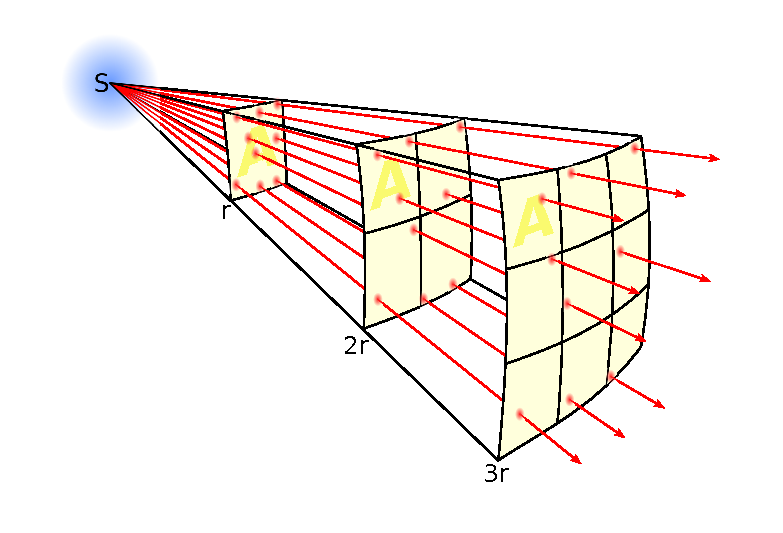
\includegraphics[width=0.8\textwidth]{./fig/photos/Inverse_square_law.eps}
    \label{fig:isl}
  \caption{An illustration of inverse square law for radioactive decay, source \protect \footnote{By Borb, CC BY-SA 3.0, https://commons.wikimedia.org/w/index.php?curid=3816716i}}
\end{figure}

\section{Interaction with matter}
As the gamma particle passes through matter, there are three possible effects that might happen:
\textbf{the photoelectric effect}, \textbf{Compton scattering} and \textbf{pair production}.

\textbf{The photoelectric effect} is typical at low energies of gamma rays. A photon undergoes an interaction with an electron that is bound in an atom. The incident photon completely disappears in this interaction. A product of this interaction is a photon.
\textbf{The Compton effect} is typical for mid-energetic gamma rays. In this process, an incident gamma photon loses energy to an atomic electron. A new lower energetic photon is emitted in a different direction (hence the frequently used term "Compton scattering").
\textbf{Pair production} is typical for high-energetic gamma rays. It is a process in which a photon of sufficient energy is converted into an electron and a positron.

\subsection{Compton effect}
The Compton effect (published in 1923 \cite{}) describes the way how a (gamma or X-ray) photon interacts with a static electron. An incident photon with wavelength $\lambda$ losses some energy to the electron. A new lower energetic photon with wavelength $\lambda^{\prime}$ is emitted under angle $\Theta$. Thanks to the law of conservation of energy and momentum, Compton derived the following equation
\begin{equation}
    \lambda^{\prime} = \lambda + \frac{h}{m_{e}c}(1-\mathrm{cos} \Theta),
\end{equation}
where $\lambda$ is the wavelength of the incident photon, $\lambda^{\prime}$ is the wavelength of the emitted photon, $h$ is the Planck constant, $m_{e}$ is the electron rest mass, $c$ is the speed of light and $\Theta$ is the scattering angle.

\begin{figure}[!h]
    \centering
    \includegraphics[width=0.3\textwidth]{./fig/photos/scattering.png}
    \label{fig:scattering}
    \caption{An illustration of Compton scattering. The incident photon interacts with the static electron. As a result, a new lower energetic photon is emitted in a direction changed by $\Theta$ as part of its energy is transferred to electron $e^{-}$. Source: \cite{baca2021gamma}}
\end{figure}

\section{Compton camera}
This effect is the fundamental principle in a sensor called a Compton camera. 
The sensor is typically composed of two main components: the scatterer and the absorber. 
The incident photon first interacts with the scatterer, where the lower energetic photon is emitted under angle $\Theta$ (thanks to the Compton effect). 
Since it is more common to measure energies instead of wavelength, we can rewrite the Compton formula as
\begin{equation}
E_{\lambda^{\prime}} = \frac{E_{\lambda}}{  1 + (E_{\lambda} / m_{e}c^{2}) (1 - \mathrm{cos} \Theta)},
\end{equation}
where $E_{\lambda}$ is the energy of the incoming photon from the source, $E_{\lambda^{\prime}}$ is the energy of the scattered photon.  
The bi-product of the interaction (electron $e_{e^{-}}$) is immediately measured in the scatterer, and its position is recorded.
Then, the scattered lower energetic photon interacts with the second layer of the sensor - the absorber. 
The photoelectric effect is witnessed while measuring the product of it - the energy of the electron $e_{\lambda^{prime}}$ and its position on the absorber.

Now we can express the scattering angle $\Theta$ as
\begin{equation}
    \Theta = \mathrm{arccos} \left (  1-\frac{m_{e}c^{2}E_{\lambda^{\prime}}}{E_{\lambda} (E_{\lambda} - E_{\lambda^{\prime}})} \right )
    \label{eq:theta}
\end{equation}

Given the measurements on the scatterer and absorber and computed scattering angle $\Theta$ using the equation \ref{eq:theta} (using known energy of the incoming photon $E_{\lambda}$), we can reconstruct a set of possible directions from where the original photon arrived. Since the Compton effect is symmetrical, the set of possible directions towards the source of ionizing radiation forms a surface of a cone.

\section{MiniPIX TPX3 sensor}
The sensor used in this work is a small CdTe event-based camera that is capable of witnessing the interactions between gamma photons and the matter of the sensor and reporting them in real time.
Unlike the traditional model of the Compton camera mentioned before, this is a single-stack detector.
In other words, there is no distinction between the scatterer and the absorber and all the measurable interactions are happening in one 14x14x2 mm block of CdTe semiconductor material.
The sensor is capable of measuring a 3D position of the interactions (and distinguishing its type) inside the detector with nanosecond resolution. 
All these features open the possibility of using it in Compton camera mode.
Technical details of the sensor are described in \cite{baca2021gamma} and \cite{baca2019timepix}.
The biggest advantage of this sensor is its small size, low weight and low power consumption.
Thanks to that, we can use this sensor on board a small UAV. 


\begin{figure}[!h]
    \centering
    \includegraphics[width=0.3\textwidth]{./fig/photos/minipix.png}
    \label{fig:minipix}
    \caption{An illustration of the detection process inside the MiniPIX TPX3 sensor. Source: \cite{baca2021gamma}}
\end{figure}

\section{Cs137}
\section{Methods for} 
